 \documentclass[12pt, a4paper]{article}
\usepackage[margin=1in]{geometry}
\usepackage[T1]{fontenc}
\usepackage[spanish]{babel}
\usepackage{graphicx}
\usepackage{fancyhdr}
\usepackage{xcolor}
\usepackage{lipsum}

% Ajuste del tamaño de \headheight
\setlength{\headheight}{34.35004pt}

% Configuración de encabezado y pie de página
\pagestyle{fancy}
\fancyhf{}
\fancyfoot[L]{\textbf{Facultad de Ciencias}}
\fancyfoot[R]{\textbf{\thepage}}
\fancyhead[R]{
\includegraphics[height=30pt]{images/uni_logo.png}}
\renewcommand{\headrulewidth}{1pt}
\renewcommand{\footrulewidth}{1pt}
\renewcommand{\footrule}{\hbox to\headwidth{\color{black}\leaders\hrule height \footrulewidth\hfill}}

\begin{document}
	
	% Página de título
	\begin{titlepage}
		\centering
		\textbf{\LARGE Universidad Nacional de Ingeniería}
		
		\vspace{1cm}
		
		\textbf{\LARGE Facultad de Ciencias}
		
		\vspace{2cm}
		
		
\includegraphics[width=7cm]{images/uni_logo.png}
		
		\vspace{2cm}
		
		\textbf{\Huge PROYECTO FORMATIVO}
		
		\vspace{2cm}
		
		\textit{\Large Integrantes:}
		
		\begin{itemize}
			\item \textbf{Luigui Jesus Cruz Sandiga} 
			\item \textbf{Martel Balvin Isaac Antonio} 
			\item \textbf{Joaquin Humberto Ramirez Caruajulca}
		\end{itemize}
		
		\vspace{0.5cm}
		
		\textit{\Large Docente:}
		
		\begin{itemize}
			\item \textbf{Americo Andres Chulluncuy Reynoso}
		\end{itemize}
		
		\vspace{2cm}
		
		
	\end{titlepage}
	
	% Nueva página para la introducción y el fundamento teórico
	\newpage
	
	% Introducción
	\section*{Introducción}
	\addcontentsline{toc}{section}{Introducción}
	
	En este proyecto formativo exploramos y comparamos dos lenguajes de programación ampliamente utilizados, Python y C++, así como dos frameworks populares para desarrollo web en Python, Django y Flask. Esta comparación se centra en identificar las fortalezas y debilidades de cada opción para ayudar en la selección adecuada según las necesidades específicas de cada proyecto.
	
	\vspace{0.5cm}
	
	% Fundamento teórico
	\section*{Fundamento Teórico}
	\addcontentsline{toc}{section}{Fundamento Teórico}
	
	% Python vs. C++
	\subsection*{Python vs. C++}
	\addcontentsline{toc}{subsection}{Python vs. C++}
	
	Python y C++ son lenguajes de programación con enfoques y características muy diferentes, cada uno con sus propias ventajas y áreas de aplicación preferidas.
	
	\vspace{0.5cm}
	
	% Subsección Python
	\subsubsection*{Python}
	\addcontentsline{toc}{subsubsection}{Python}
	
	\textbf{Ventajas:}
	\begin{itemize}
		\item Sintaxis sencilla y legible.
		\item Amplia variedad de bibliotecas y frameworks.
		\item Ideal para desarrollo rápido y prototipado.
	\end{itemize}
	
	\textbf{Desventajas:}
	\begin{itemize}
		\item Rendimiento relativamente menor en comparación con C++.
		\item Gestión de memoria menos eficiente.
	\end{itemize}
	
	\vspace{0.3cm}
	
	% Imagen para Python vs. C++
	\begin{figure}[ht]
		\centering
		
\includegraphics[width=0.6\textwidth]{images/python_vs_cpp.png}
		\caption{Comparación Python vs. C++}
		\label{fig:python_cpp}
	\end{figure}
	
	\vspace{0.5cm}
	
	% Subsección C++
	\subsubsection*{C++}
	\addcontentsline{toc}{subsubsection}{C++}
	
	\textbf{Ventajas:}
	\begin{itemize}
		\item Alto rendimiento y control cercano al hardware.
		\item Eficiente gestión de memoria.
		\item Ampliamente utilizado en sistemas embebidos y juegos.
	\end{itemize}
	
	\textbf{Desventajas:}
	\begin{itemize}
		\item Sintaxis más compleja y propensa a errores.
		\item Curva de aprendizaje más pronunciada.
	\end{itemize}
	
	\vspace{0.3cm}
	
	% Imagen para Flask vs. Django
	\begin{figure}[ht]
		\centering
		
\includegraphics[width=0.6\textwidth]{images/django_vs_flask.png}
		\caption{Comparación Flask vs. Django}
		\label{fig:flask_django}
	\end{figure}
	
	\vspace{0.5cm}
	
	% Django vs. Flask
	\subsection*{Django vs. Flask}
	\addcontentsline{toc}{subsection}{Django vs. Flask}
	
	Django y Flask son frameworks para desarrollo web en Python, cada uno con características únicas que los hacen adecuados para diferentes tipos de proyectos.
	
	\vspace{0.5cm}
	
	% Subsección Django
	\subsubsection*{Django}
	\addcontentsline{toc}{subsubsection}{Django}
	
	\textbf{Ventajas:}
	\begin{itemize}
		\item Framework completo con muchas funcionalidades integradas.
		\item Facilita el desarrollo rápido y estructurado de aplicaciones complejas.
		\item Ideal para proyectos que requieren seguridad y escalabilidad.
	\end{itemize}
	
	\textbf{Desventajas:}
	\begin{itemize}
		\item Puede ser excesivo para proyectos pequeños o simples.
		\item Curva de aprendizaje más pronunciada que Flask.
	\end{itemize}
	
	\vspace{0.3cm}
	
	% Subsección Flask
	\subsubsection*{Flask}
	\addcontentsline{toc}{subsubsection}{Flask}
	
	\textbf{Ventajas:}
	\begin{itemize}
		\item Ligero y flexible.
		\item Fácil de aprender y comenzar a usar.
		\item Ideal para proyectos pequeños y prototipos rápidos.
	\end{itemize}
	
	\textbf{Desventajas:}
	\begin{itemize}
		\item Requiere más configuración manual para funcionalidades avanzadas.
		\item Menos integrado que Django en términos de características integradas.
	\end{itemize}
	
	\vspace{0.5cm}
	
% Funciones en Python
\subsubsection*{Funciones en Python}
\addcontentsline{toc}{subsubsection}{Funciones en Python}

\begin{figure}[ht]
	\centering
	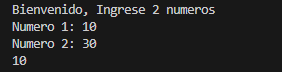
\includegraphics[width=0.6\textwidth]{images/funciones_python.png}
	\label{fig:funciones_python}
\end{figure}

\begin{verbatim}

	def mcd(numero1, numero2):
	if numero1 == 0:
	return numero2
	return mcd(numero2 % numero1, numero1)
		if __name__ == '__main__':
	print("Bienvenido, Ingrese 2 numeros")
	
	num1 = int(input("Numero 1: "))
	num2 = int(input("Numero 2: "))
	print(mcd(num1, num2))
\end{verbatim}

\vspace{0.5cm}

% Cadenas en Python
\subsubsection*{Cadenas en Python}
\addcontentsline{toc}{subsubsection}{Cadenas en Python}

\begin{figure}[ht]
	\centering
	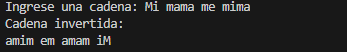
\includegraphics[width=0.6\textwidth]{images/cadenas_python.png}
	\label{fig:cadenas_python}
\end{figure}

\begin{verbatim}
	def invertCad(cad):
	newCad = ""
	for i in cad:
	newCad = i + newCad
	return newCad
	
	if __name__ == '__main__':
	cadena = input("Ingrese una cadena: ")
	print("Cadena invertida:")
	print(invertCad(cadena))
	
	
\end{verbatim}
\vspace{0.5cm}

% Diccionarios en Python
\subsubsection*{Diccionarios en Python}
\addcontentsline{toc}{subsubsection}{Diccionarios en Python}

\begin{figure}[ht]
	\centering
	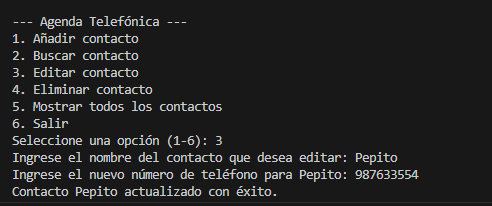
\includegraphics[width=0.6\textwidth]{images/diccionarios_python.png}
	\label{fig:diccionarios_python}
\end{figure}

\begin{verbatim}
	# Definición de la agenda telefónica como un diccionario
	agenda = {}
	
	# Función para mostrar el menú
	def mostrar_menu():
	print("\n--- Agenda Telefónica ---")
	print("1. Añadir contacto")
	print("2. Buscar contacto")
	print("3. Editar contacto")
	print("4. Eliminar contacto")
	print("5. Mostrar todos los contactos")
	print("6. Salir")
	
	# Función para añadir un contacto
	def añadir_contacto():
	nombre = input("Ingrese el nombre del contacto: ")
	telefono = input("Ingrese el número de teléfono: ")
	agenda[nombre] = telefono
	print(f"Contacto {nombre} añadido con éxito.")
	
	# Función para buscar un contacto
	def buscar_contacto():
	nombre = input("Ingrese el nombre del contacto que desea buscar: ")
	if nombre in agenda:
	print(f"El número de teléfono de {nombre} es {agenda[nombre]}.")
	else:
	print(f"El contacto {nombre} no se encuentra en la agenda.")
	
	# Función para editar un contacto
	def editar_contacto():
	nombre = input("Ingrese el nombre del contacto que desea editar: ")
	if nombre in agenda:
	telefono = input(f"Ingrese el nuevo número de teléfono para {nombre}: ")
	agenda[nombre] = telefono
	print(f"Contacto {nombre} actualizado con éxito.")
	else:
	print(f"El contacto {nombre} no se encuentra en la agenda.")
	
	# Función para eliminar un contacto
	def eliminar_contacto():
	nombre = input("Ingrese el nombre del contacto que desea eliminar: ")
	if nombre in agenda:
	del agenda[nombre]
	print(f"Contacto {nombre} eliminado con éxito.")
	else:
	print(f"El contacto {nombre} no se encuentra en la agenda.")
	
	# Función para mostrar todos los contactos
	def mostrar_todos_los_contactos():
	if agenda:
	print("\n--- Lista de Contactos ---")
	for nombre, telefono in agenda.items():
	print(f"Nombre: {nombre}, Teléfono: {telefono}")
	else:
	print("La agenda está vacía.")
	
	# Función principal
	def main():
	while True:
	mostrar_menu()
	opcion = input("Seleccione una opción (1-6): ")
	if opcion == '1':
	añadir_contacto()
	elif opcion == '2':
	buscar_contacto()
	elif opcion == '3':
	editar_contacto()
	elif opcion == '4':
	eliminar_contacto()
	elif opcion == '5':
	mostrar_todos_los_contactos()
	elif opcion == '6':
	print("Saliendo de la agenda. ¡Hasta luego!")
	break
	else:
	print("Opción no válida. Inténtelo de nuevo.")
	
	# Ejecución del programa principal
	if __name__ == "__main__":
	main()	
	
	
\end{verbatim}

% Archivos en Python
\subsubsection*{Archivos en Python}
\addcontentsline{toc}{subsubsection}{Archivos en Python}

\begin{figure}[ht]
	\centering
	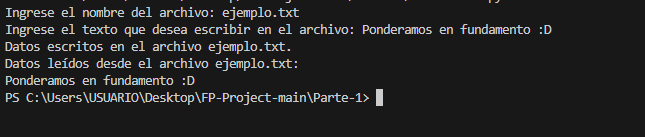
\includegraphics[width=0.6\textwidth]{images/archivos_python.png}
	\label{fig:archivos_python}
\end{figure}

\begin{verbatim}
	def escribir_datos(nombre_archivo, datos):
	try:
	with open(nombre_archivo, 'w') as archivo:
	archivo.write(datos)
	print(f"Datos escritos en el archivo {nombre_archivo}.")
	except Exception as e:
	print(f"Ocurrió un error al escribir en el archivo: {e}")
	def leer_datos(nombre_archivo):
	try:
	with open(nombre_archivo, 'r') as archivo:
	datos = archivo.read()
	print(f"Datos leídos desde el archivo {nombre_archivo}:")
	print(datos)
	return datos
	except Exception as e:
	print(f"Ocurrió un error al leer el archivo: {e}")
	return None	
	# Solicitar al usuario el nombre del archivo y los datos a escribir
	nombre_archivo = input("Ingrese el nombre del archivo: ")
	datos_a_escribir = input("Ingrese el texto que desea escribir en el archivo: ")
	
	# Escribir datos en el archivo
	escribir_datos(nombre_archivo, datos_a_escribir)
	
	# Leer datos desde el archivo
	datos_leidos = leer_datos(nombre_archivo)
	
\end{verbatim}

% Clases en Python
\subsubsection*{Clases en Python}
\addcontentsline{toc}{subsubsection}{Clases en Python}

\begin{figure}[ht]
	\centering
	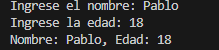
\includegraphics[width=0.6\textwidth]{images/clases_python.png}
	\label{fig:clases_python}
\end{figure}

\begin{verbatim}
	class Persona:
	def __init__    (self, nombre, edad): #No es  necesario agregar el __init__, pero es una práctica común y recomendada en Python para inicializar los atributos de una clase.
	self.nombre = nombre
	self.edad = edad
	
	def mostrar_datos(self):
	print(f"Nombre: {self.nombre}, Edad: {self.edad}")
	
	# Solicitar datos al usuario
	nombre = input("Ingrese el nombre: ")
	edad = int(input("Ingrese la edad: "))
	
	# Crear una instancia de la clase Persona con los datos ingresados
	persona1 = Persona(nombre, edad)
	
	# Mostrar los datos
	persona1.mostrar_datos()
	
\end{verbatim}

	
% Parte 2
\subsection*{Parte 2}
\addcontentsline{toc}{subsection}{Parte 2}

\vspace{0.5cm}

% Calculadora en Python
\subsubsection*{Calculadora en Python}
\addcontentsline{toc}{subsubsection}{Calculadora en Python}

\begin{figure}[ht]
	\centering
	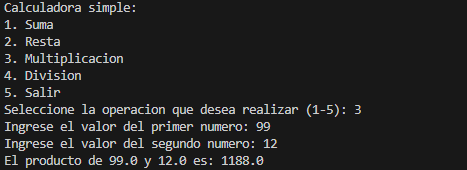
\includegraphics[width=0.6\textwidth]{images/calculadora_python.png}
	\label{fig:calculadora_python}
\end{figure}

\begin{verbatim}
	
	def suma(x, y):
	return x + y
	
	def resta(x, y):
	return x - y
	
	def producto(x, y):
	return x * y
	
	def division(x, y):
	if y != 0:
	return x / y
	else:
	return "ERROR! No se puede dividir entre 0."
	
	def calculadora():
	while True:
	print("Calculadora simple: ")
	print("1. Suma")
	print("2. Resta")
	print("3. Multiplicacion")
	print("4. Division")
	print("5. Salir")
	
	op = input("Seleccione la operacion que desea realizar (1-5): ")
	
	while op not in ['1', '2', '3', '4', '5']:
	print("Entrada no valida. Intente nuevamente.")
	op = input("Seleccione la operacion que desea realizar (1-5): ")
	
	if op == '5':
	print("Saliendo...")
	break
	
	num1 = float(input("Ingrese el valor del primer numero: "))
	num2 = float(input("Ingrese el valor del segundo numero: "))
	
	if op == '1':
	resultado = suma(num1, num2)
	print(f"La suma de {num1} y {num2} es: {resultado}")
	elif op == '2':
	resultado = resta(num1, num2)
	print(f"La diferencia entre {num1} y {num2} es: {resultado}")
	elif op == '3':
	resultado = producto(num1, num2)
	print(f"El producto de {num1} y {num2} es: {resultado}")
	elif op == '4':
	resultado = division(num1, num2)
	print(f"El cociente entre {num1} y {num2} es: {resultado}")
	
	calculadora()
	
\end{verbatim}


% Parte 3: Aplicativo web
\subsection*{Parte 3: Aplicativo web}
\addcontentsline{toc}{subsection}{Parte 3: Aplicativo web}

En esta sección, se presentará la estructura y funcionamiento de un aplicativo web desarrollado con Django. A continuación, se muestran ejemplos de código y capturas de pantalla del archivo `models.py` ,asi como otros componentes relevantes.

% Imagen del archivo models.py
\begin{figure}[ht]
	\centering
	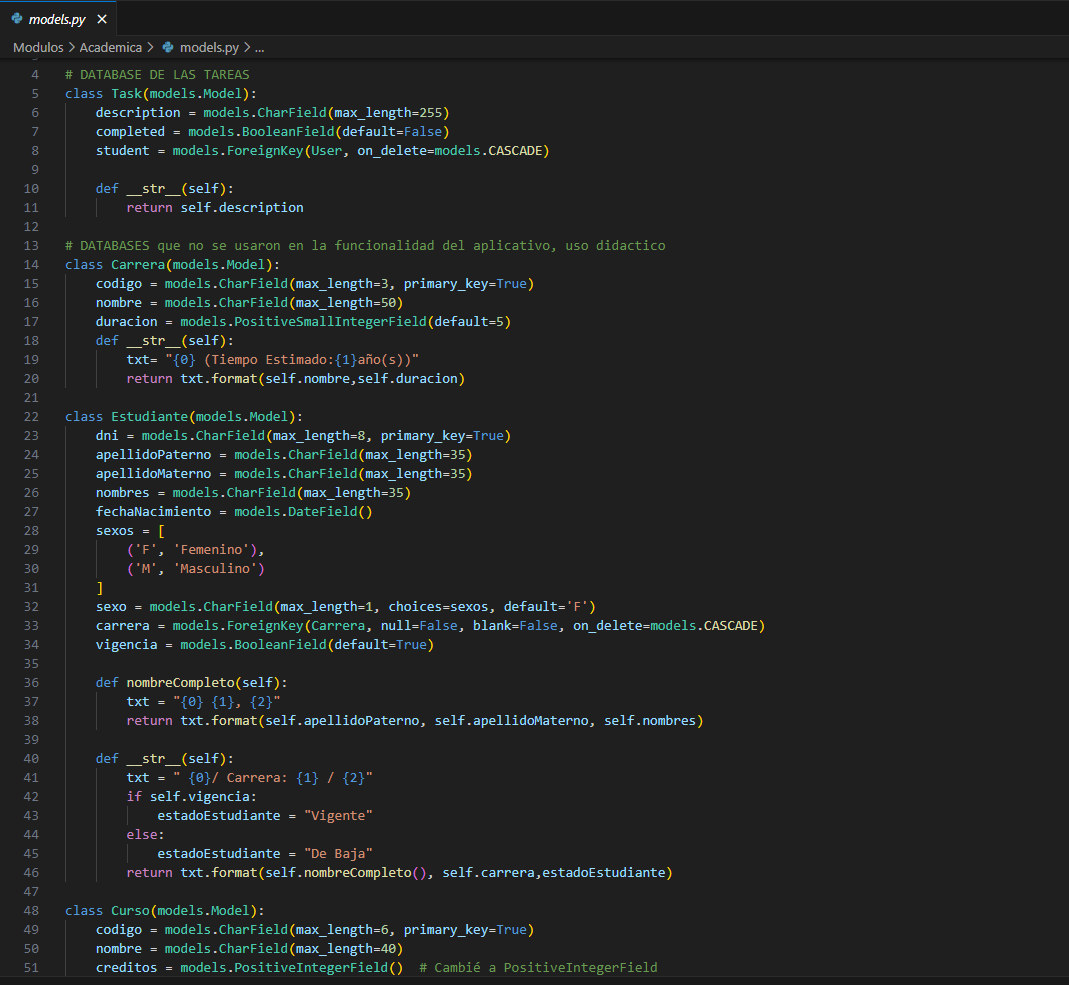
\includegraphics[width=0.8\textwidth]{images/models1.png}
	\caption{Parte 1 del archivo models.py}
	\label{fig:models1}
\end{figure}

\begin{figure}[ht]
	\centering
	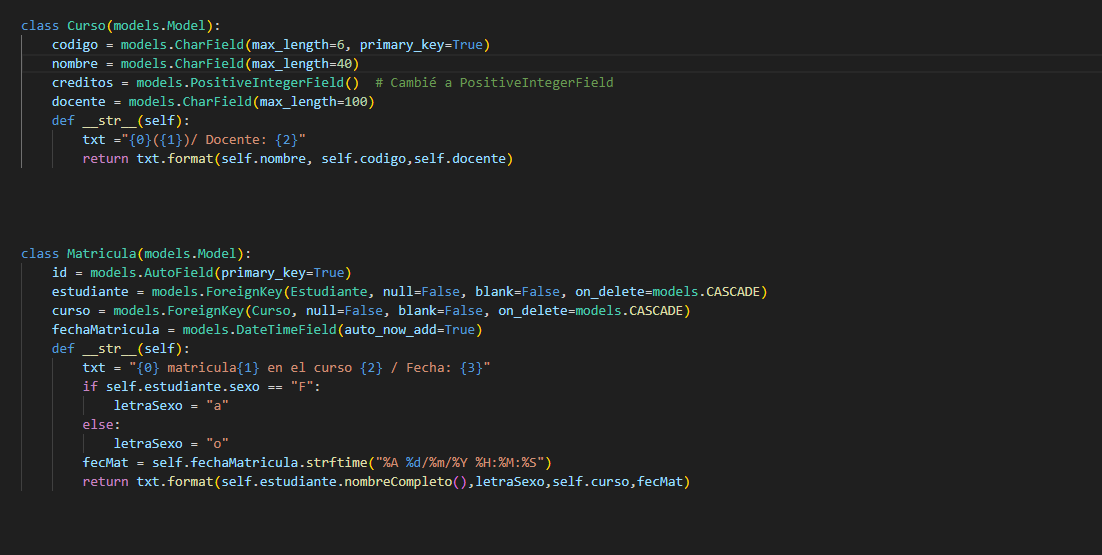
\includegraphics[width=0.8\textwidth]{images/models2.png}
	\caption{Parte 2 del archivo models.py}
	\label{fig:models2}
\end{figure}

% Imagen del archivo views.py
\begin{figure}[ht]
	\centering
	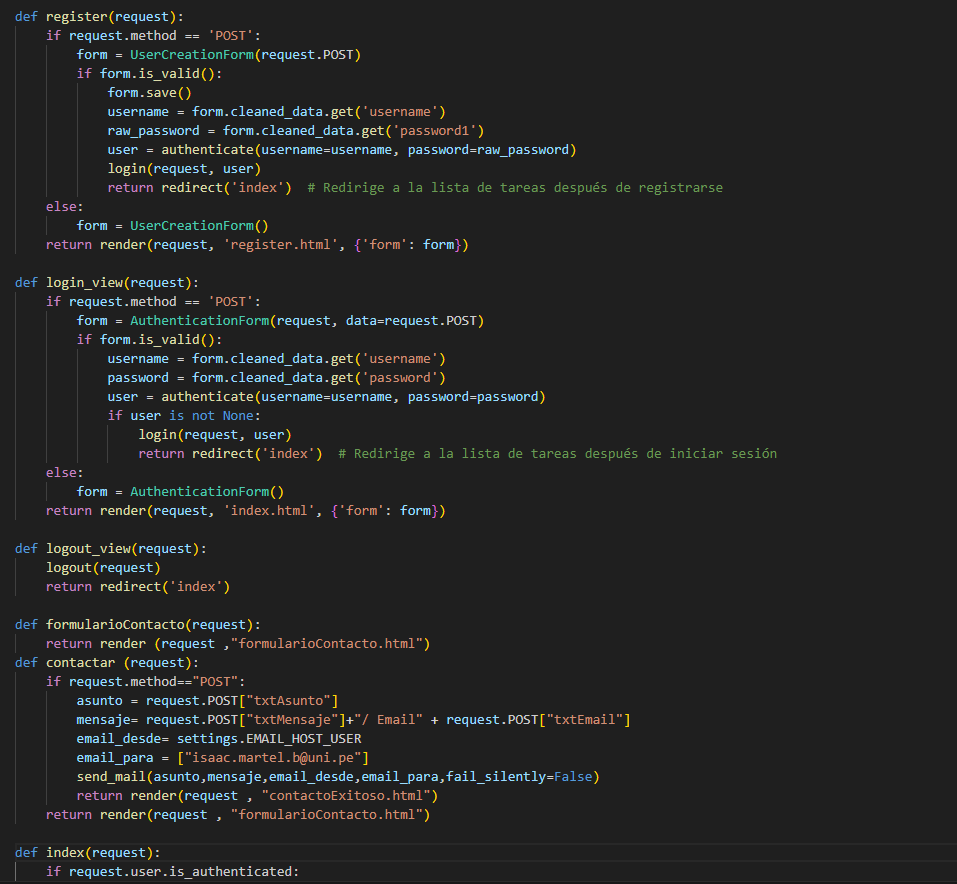
\includegraphics[width=0.8\textwidth]{images/views1.png}
	\caption{Código del archivo views1.py}
	\label{fig:views1}
\end{figure}

\begin{figure}[ht]
	\centering
	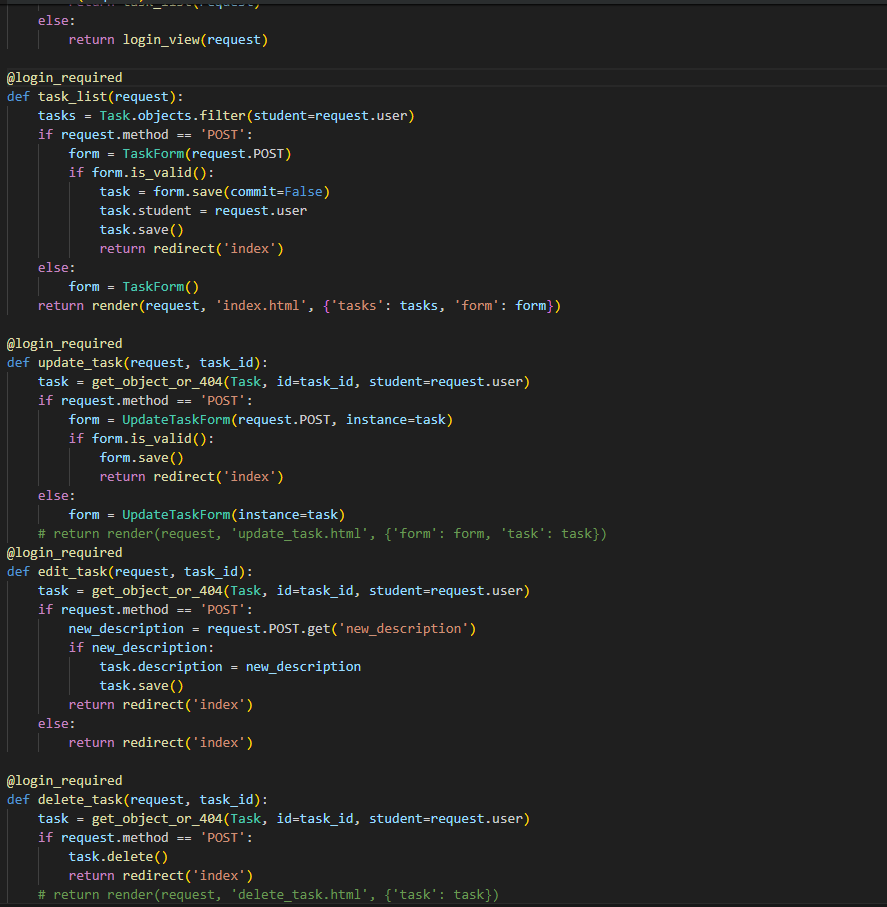
\includegraphics[width=0.8\textwidth]{images/views2.png}
	\caption{Código del archivo views2.py}
	\label{fig:views2}
\end{figure}

% Imagen del archivo urls.py
\begin{figure}[ht]
	\centering
	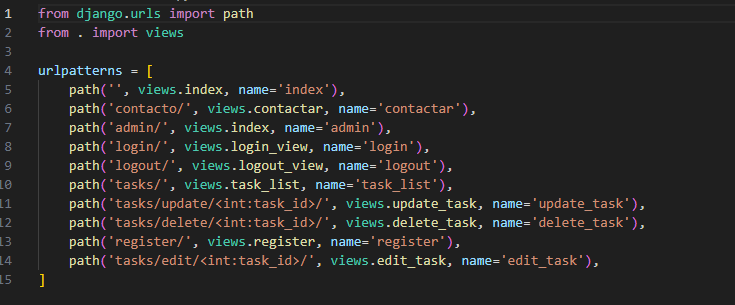
\includegraphics[width=0.8\textwidth]{images/urls.png}
	\caption{Código del archivo urls.py}
	\label{fig:urls}
\end{figure}

% Imagen de la interfaz web
\begin{figure}[ht]
	\centering
	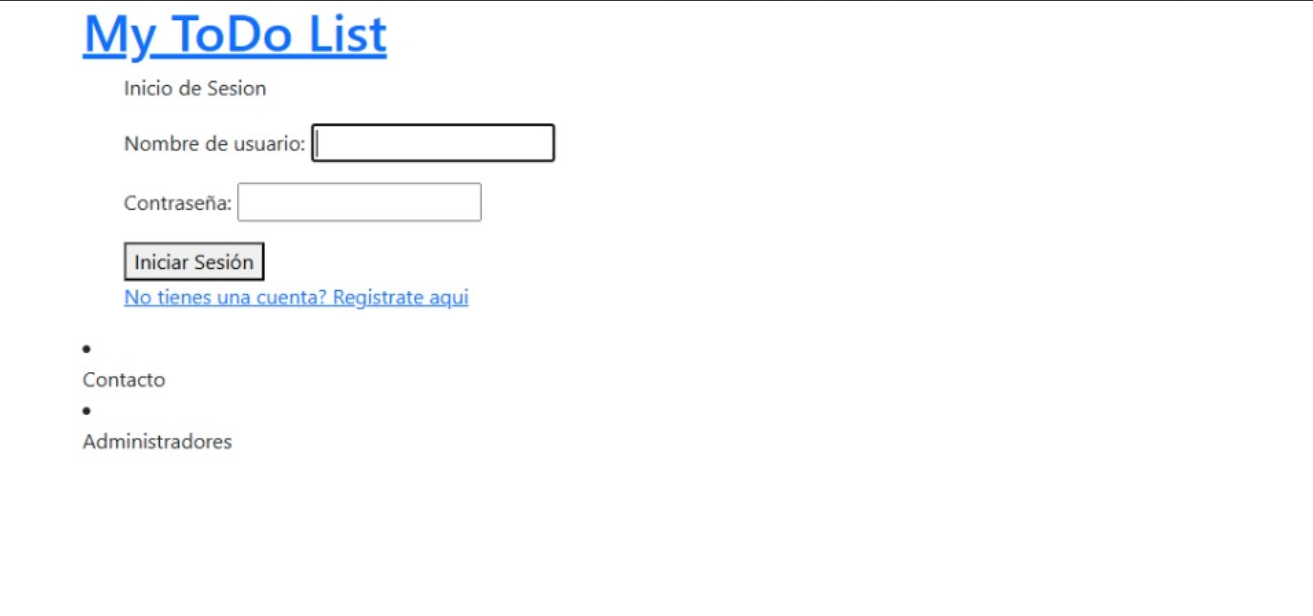
\includegraphics[width=0.8\textwidth]{images/interface1.png}
	\caption{Captura de la interfaz web}
	\label{fig:interface1}
\end{figure}

\begin{figure}[ht]
	\centering
	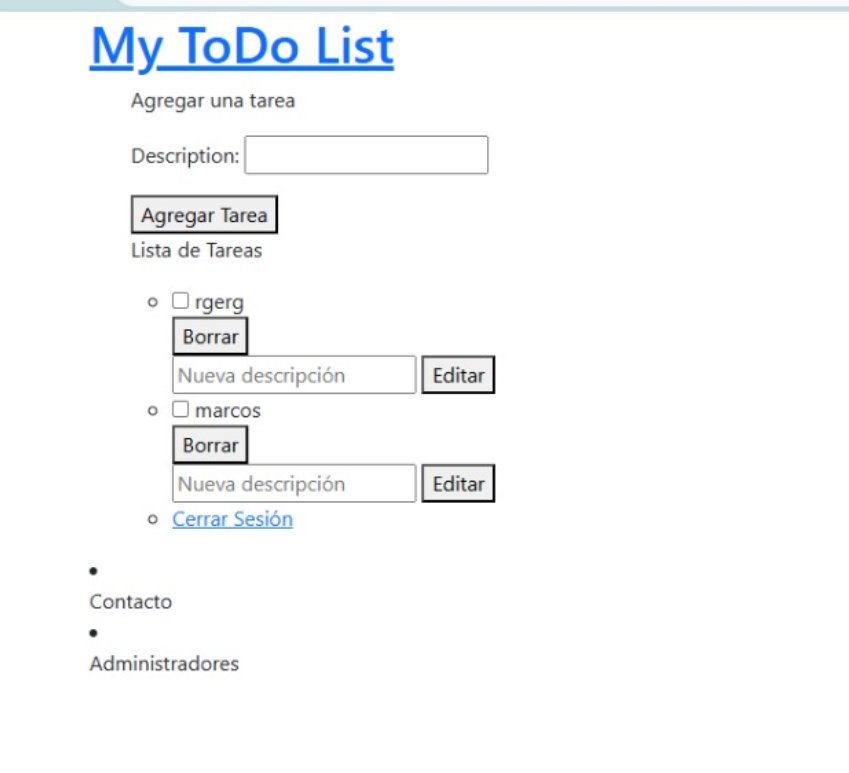
\includegraphics[width=0.8\textwidth]{images/interface2.png}
	\caption{Captura 2 de la interfaz web}
	\label{fig:interface2}
\end{figure}
	

	% Conclusión
	\section*{Conclusión}
	\addcontentsline{toc}{section}{Conclusión}
	
	En conclusión, tanto en el ámbito de los lenguajes de programación como en los frameworks para desarrollo web, la elección entre Python y C++, y entre Django y Flask, depende en gran medida de las necesidades específicas del proyecto. Cada opción tiene sus puntos fuertes y áreas de aplicación preferidas, lo que permite a los desarrolladores tomar decisiones informadas para maximizar la eficiencia y la efectividad en el desarrollo de software.
	
\end{document}












